\begin{figure*}[t]
  \centering
  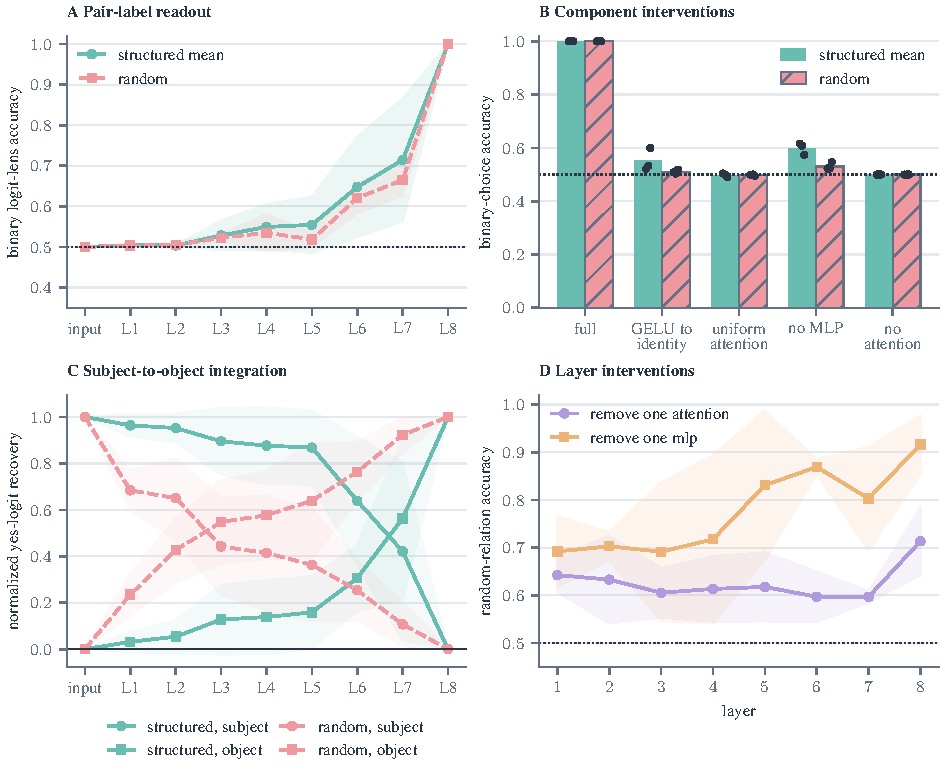
\includegraphics[width=1.0\textwidth]{goal2_raw_transformer_mechanism.pdf}
  \caption{In Experiment~B, the memorized random relation relies on distributed
  nonlinear computation across the eight transformer layers (means $\pm$ 1 SD
  over three seeds). \textbf{A:} A layerwise logit lens tracks when the random
  answer becomes linearly readable across the eight layers. \textbf{B:} Global
  interventions on GELU activations, attention routing, MLP outputs, or
  attention outputs degrade accuracy on both structured and random relations.
  \textbf{C:} Residual-stream patching shows relational information shifting
  from the subject position to the object position across layers. \textbf{D:}
  Ablating any single attention or MLP sublayer impairs random-relation recall,
  showing that the lookup is distributed across layers.}
  \label{fig:goal2-mechanism}
\end{figure*}

\section{The memorized random lookup uses distributed nonlinear computation}
\label{sec:mechanism}

How does the eight-layer transformer in Experiment~B achieve 99.98\% accuracy on
$\Rrnd$ when a linear regression on the embeddings explains only 37.5\% of its
target centroid variance? We apply causal interventions and layerwise probing to
identify how the forward pass computes the memorized lookup
(Figure~\ref{fig:goal2-mechanism}).

With trained weights fixed, replacing GELU activations with the identity
function reduces random-relation accuracy from nearly 100\% to 51\%. Making
attention weights uniform or ablating all attention or MLP outputs likewise
reduces accuracy to near chance (50\%; Figure~\ref{fig:goal2-mechanism}B). The
memorized lookup therefore depends on nonlinear MLP activations and
content-dependent attention routing.

A layerwise logit lens shows that the correct yes/no answer for $\Rrnd$ becomes
linearly decodable from the residual stream only in the final transformer layer
(Figure~\ref{fig:goal2-mechanism}A). Nevertheless, ablating any single attention
or MLP sublayer in earlier layers degrades accuracy
(Figure~\ref{fig:goal2-mechanism}D), showing that intermediate layers
incrementally construct the lookup representation.

Residual-stream patching across layers tracks how information moves between
token positions (Figure~\ref{fig:goal2-mechanism}C; metric details in
Appendix~\ref{app:metrics}). Patching the clean subject representation into a
corrupted prompt recovers the answer margin in early layers, whereas patching
the object position recovers the margin in later layers, consistent with
attention routing subject information to the final object position where the
yes/no prediction is emitted. Because global component ablations impair both
structured and random relations (Figure~\ref{fig:goal2-mechanism}B), both rely
on nonlinear forward computation; what distinguishes them is whether the
underlying entity embeddings organize into a linearly decodable geometry.

